\documentclass{llncs}

\usepackage[utf8]{inputenc}
\usepackage{booktabs}
\usepackage{tabularx}
\usepackage{graphicx}
\usepackage{ragged2e} 
\renewcommand{\arraystretch}{1.2} 


\usepackage[backend=biber,style=numeric,citestyle=ieee,doi=false,isbn=false,arxiv=false]{biblatex}

\AtEveryBibitem{\clearfield{publisher}}
\AtEveryBibitem{\clearfield{editor}}
% Fix Mendely URL stuff 1
\AtEveryBibitem{\ifentrytype{article}{\clearfield{url}}{}}
\AtEveryBibitem{\ifentrytype{inproceedings}{\clearfield{url}}{}}
\AtEveryBibitem{\ifentrytype{book}{\clearfield{url}}{}}
\AtEveryBibitem{\ifentrytype{incollection}{\clearfield{url}}{}}
% Fix Mendeley URL stuff 2
\DeclareSourcemap{
    \maps{
        \map{ % Replaces '{\_}', '{_}' or '\_' with just '_'
            \step[fieldsource=url,
                  match=\regexp{\{\\\_\}|\{\_\}|\\\_},
                  replace=\regexp{\_}]
        }
        \map{ % Replaces '{'$\sim$'}', '$\sim$' or '{~}' with just '~'
            \step[fieldsource=url,
                  match=\regexp{\{\$\\sim\$\}|\{\~\}|\$\\sim\$},
                  replace=\regexp{\~}]
        }
    }
}

% \addbibresource{ref.bib} % Overleaf
\addbibresource{../../bib/library.bib} % local

\usepackage{todonotes}
\newcommand{\dha}[1]{\todo[linecolor=yellow,backgroundcolor=yellow!25,bordercolor=yellow,inline,caption={}]{Comment by Dominik: #1}}
\newcommand{\todha}[1]{\todo[linecolor=yellow,backgroundcolor=yellow!25,bordercolor=yellow,inline,caption={}]{Todo for Dominik: #1}}

\begin{document}


\title{Towards Safer Smart Contracts: A Survey of Languages and Verification Methods}
%\author{Dominik Harz}
%\institute{IC3RE \\ Imperial College London \\ \email{d.harz@imperial.ac.uk}}



\maketitle

\begin{abstract}
With a market capitalisation of over USD 205 billion in just under ten years, public distributed ledgers have experienced significant adoption.
Apart from novel consensus mechanisms, their success is also accountable to smart contracts. 
These programs allow distrusting parties to enter agreements that are executed autonomously.
However, implementation issues in smart contracts caused severe losses to the users of such contracts.
Significant efforts are taken to improve their security by introducing new programming languages and advance verification methods.
We provide an overview of those efforts in two parts.
First, we introduce several smart contract languages focussing on security features.
To that end, we present an overview concerning paradigm, type, instruction set, semantics, and metering.
Second, we survey verification tools and methods for smart contract and distributed ledgers. 
Accordingly, we introduce their verification approach, level of automation, coverage, and supported languages.
Last, we present future research directions including formal semantics, verified compilers, and automated verification.
\end{abstract}

\section{Introduction}
The idea of contracts between independent parties goes back to autonomous agents using a network of agents to solve tasks distributed and based on individual contracts as presented in the contract net protocol (CNP) \cite{Smith1980}.
The idea was further elaborated, with a focus on minimising and ideally excluding the need for trust in either party, by Szabo coining the term ``smart contract'' \cite{Szabo1997}.
Significant work has been directed towards creating languages and framework for electronic contracts even before the inception of distributed ledgers, for example, \cite{Andersen2006,Kyas2008,Xu2004}.
% However, distributed ledgers are the ones facilitating the wide-spread adoption of electronic contracts.


Smart contracts based on distributed ledgers combine two unique properties: anyone can freely create such contracts for the whole world to interact with, while each line of code (LoC) might affect a significant amount of currency (in the range of millions of USD per LoC).
These contracts allow economic interactions between different parties without the need to trust one another.
This includes contracts for financial services, notaries, games, wallets, or libraries \cite{Bartoletti2017}.
Further, smart contracts are the enabler of protocols build on top of distribued legers including, for example, Lightning \cite{Poon2016}, Plasma \cite{Poon2017}, Polkadot \cite{Wood2017}, and TrueBit \cite{Teutsch2017}.
However, security incidents caused by software bugs has lead to severe losses as in the infamous The DAO incident \cite{Daian2016}, and Parity multi-sig vulnerabilities \cite{Breidenbach2017Parity,ParityTech2017}. 


Significant efforts are taken to prevent such future incidents. 
High-level programming languages are introduced to encourage safe programming practices, for example  \cite{Hirai2018Bamboo,Ethereum2018Vyper,Schrans2018}.
Languages for distributed virtual machines that allow for easy verification are realised, for example \cite{Sergey2018,DynamicLedgerSolutions2017,Popejoy2017,Kasampalis2018}.
Tools for analysing source code by symbolic modelling and execution, for example \cite{Luu2016,Tsankov2017,Kalra2018,Albert2018} as well as formal semantics and verification, for example \cite{Bhargavan2016,Hildenbrandt2017,Hirai2017}, are developed.

\paragraph{Contribution:} The amount of new languages, approaches for verification, and applicability of verification methods becomes quickly opaque. Due to the practical impact of these approaches to real-world smart contracts, we present a literature survey on current languages and verification efforts.
We contribute an overview of contract languages including a classification of language paradigm, essential security features, and state of implementation\footnote{As of September 2018.}.
Further, we describe different efforts to verify software including model- and proof-based methods. This includes an analysis of the applicability of different techniques, limitations, and current availability of methods.

\paragraph{Structure:} The remainder of our article is structured as follows. Section \ref{background} introduces the background of contracts and languages to express them. We present an overview and a classification of languages in section \ref{languages}. Similarly, verification approaches are examined in section \ref{verification}. Our results are discussed including related work in section \ref{discuss}. We conclude in section \ref{conclusion}.

\section{Safer smart contracts}
\label{background}

% Electronic contracts have early beginnings in the AI and agent community where they are used as a basis for interaction \cite{Smith1980}. Moreover, electronic contracts are discussed and used for automating or encoding traditional contracts in organisational and business contexts \cite{Hvitved2010}. Specifically, Ricardian contracts are oft-cited as they introduce encoding natural language contracts into electronic contracts that can be executed by computer systems \cite{Grigg2004}. Later, electronic contracts are applied to enforce agreements between mutually untrusted entities \cite{Szabo1997}.


% If everyone trusted each other, contracts would not be a necessity.
% However, a significant amount of interaction is conducted between untrusted or semi-trusted parties.

\subsection{Contracts and trust}

Contracts are a requirement resulting from an inherent lack of trust between parties.
Electronic contracts have been considered as a way to encode legal contracts (e.g. Ricardian contracts \cite{Grigg2004}) in a Domain Specific Language (DSL). 
They can be processed digitally enabling automated business processes.
How to encode contracts has been surveyed in \cite{Hvitved2010}. 
The author list 13 different requirements that a language needs to fulfil.
He found that those languages can be roughly categorised into four different formalisms including deontic logic, event-condition-action, action-trace, and others.
Most of these languages do not have formal semantics except for \cite{Andersen2006,Kyas2008,Xu2004}.
Underlying those languages is often the assumption that parties adhere to the contract.
Rather than enforcing contracts through a consensus protocol, those systems monitor compliance of participants in the form of norms (permissions, obligations, and prohibitions), e.g.\ \cite{Kyas2008}.

Smart contracts execute agreements on a distributed ledger like Bitcoin or Ethereum \cite{Nakamoto2008,Buterin2013}.
The consensus protocol of the ledger ensures that the smart contract is executed correctly and only results agreed by a majority are accepted.
Consensus protocols enable mutually \emph{distrusting parties} to create contracts and interact.
% Likewise, parties that have a form of \emph{trusted relationship} can utilise smart contracts on a ledger with stronger trust assumptions.
% This can be beneficial since, e.g. transaction rates can be higher and fees (if any) lower.
However, there is a caveat with distributed ledgers and their consensus protocols.
Results of contracts need to be fully deterministic so that each party participating in the consensus protocol reaches the same conclusion with a common set of inputs.

% Smart contracts can be used to encode legal contracts, much like the equivalent electronic contract systems \cite{Neal.2003,Governatori2006,Clack2016}.
% Yet, smart contracts do not necessarily have to have a ``real-world'' legal contract equivalent \cite{Szabo1997,Nakamoto2008,Buterin2013}. 
% In the legal context, disputes can be resolved in the traditional legal system of the original contract.
% Where a smart contract does not have a related legal contract, dispute resolution must be included in the protocol of the contract.
% If this is not the case, disputes might not be resolved.
% Projects like Mattereum try to bridge the gap \cite{Gupta}.
% Nonetheless, in both settings, the contract languages play a crucial role.

\subsection{Languages for contracts}

Smart contracts need a low-level language that allows deterministic execution. 
A high-level language can make it easier for developers to create new contracts and reason about existing contracts.
In software development, having different sets of languages is a conventional process.
Similarly, we can distinguish three different levels of languages for smart contracts.

\begin{itemize}
\item \emph{High-level languages} should provide a way to express the desired contracts. These languages can have a wide range of possible paradigms including procedural, logic, functional, or object-oriented. Depending on the use case and intended use of the language, the paradigm can be adjusted. Moreover, multiple high-level languages can exist in parallel to be executed on the same ledger. Examples for high-level languages are Solidity \cite{Ethereum2018Solidity} and Liquidity \cite{OCamlProSAS2018}.
\item \emph{Intermediary representations (IR)} are between low-level and high-level languages. IRs can be used to write programs to reason about properties (like safety or liveness) or optimising code. Examples include Simplicity \cite{OConnor2017} and Scilla \cite{Sergey2018}.
\item \emph{Low-level languages} need to implement the contract in a deterministic way so that it can be executed on a distributed virtual machine (VM). Examples include Bitcoin Script \cite{BitcoinWiki2018Script} and EVM bytecode \cite{Wood2014}.
\end{itemize}

Additionally, the \emph{distributed ledger} plays a vital role in the design of the language. Bitcoin and others implement a UTXO model \cite{Nakamoto2008,Covaci2018}, where contracts are restricted to one transaction. Account-based ledgers have a global state and contracts can typically access this state. 
However, this can introduce security issues when dependencies on the global state are introduced within the contract that can be influenced by parties outside of the contract (typically miners). Other issues revolve around calling into other, possibly faulty or unpredictable, contracts.

% \subsection{Contract verification}

%\subsection{Survey objective}
%Smart contracts potentially handle large amounts of money.
%Hence, keeping them safe requires efforts on different levels.
%We summarise the efforts taken to create safe smart contracts by answering the following research question.
%
%\paragraph{\textbf{RQ:}} How can languages and verification methods contribute to safer smart contracts?
%
%
%\paragraph{} In detail, we present relevant previous work according to languages and verification tools.
%High-level languages can encourage secure programming principles that reduce the number of bugs a programmer introduces.
%IR and low-level languages can be designed to simplify program analysis and verification.
%Verification tools can analyse specific properties or full contracts by using representative models or proof methods.
%% Their impact can be promoted by full coverage and ease of use.
%Last, verified compilers are a practice to allow reasoning of programs at a higher level and safe execution at a lower level.
% Design by contract \cite{Meyer1992}


\section{Contract languages}
\label{languages}

A range of languages for smart contracts exists. Figure \ref{fig:lang} gives an overview of the implementation levels of languages.
The approach in (A) is often used to allow program optimisation and verification (e.g. \cite{Lattner2004}). 
Among the projects that follow this approach are the future Ethereum development with Yul \cite{EthereumFoundation2018IULIA}, and Tezos with Liquidity \cite{OCamlProSAS2018} and Michelson \cite{DynamicLedgerSolutions2017}.
Likewise, Scilla based on Coq is intended to represent an IR that is targeted by more general languages and compiles down to be executed on a distributed VM \cite{Sergey2018}.

Smart contracts are a comparably new discipline with Bitcoin being ten years old and Ethereum a bit older than three years.
Hence, in the early stages smart contracts were designed differently as represented by (B).
Bitcoin and Bitcoin Script \cite{BitcoinWiki2018Script} skip any high-level language altogether and programmers need to write code directly in the low-level stack-based language.
Ethereum, on the other hand, offers multiple high-level languages like Solidity \cite{Ethereum2018Solidity} and Vyper \cite{Ethereum2018Vyper}.
These languages compile directly to EVM bytecode. 
Since Solidity 0.4.23, an IR called Yul (formlerly IULIA and JULIA) is available for Solidity \cite{EthereumFoundation2018IULIA}.

\begin{figure}
\label{fig:lang}
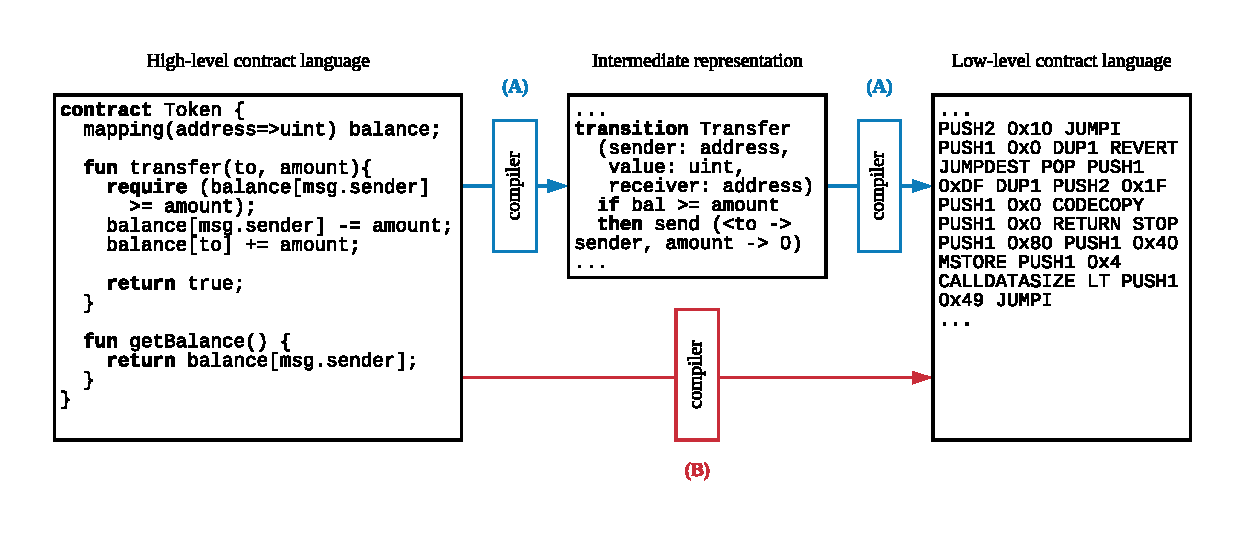
\includegraphics[width=\textwidth]{fig/Language.pdf}
\caption{Different levels of smart contract languages with syntax closely resembled to Solidity (high-level), Scilla (IR), and EVM bytecode (low-evel). (A) represents an optimised version of compiling high-level languages towards the bytecode that allows for example for verification of the IR contract and code optimisations, for example envisioned by \cite{Sergey2018,OCamlProSAS2018}. (B) represents the straightforward compilation from high-level language to bytecode representation as currently employed by Solidity and the EVM \cite{Ethereum2018Solidity,Wood2014}.}
\end{figure}


\subsection{Summary}
The overview we present in table \ref{tab:high-level} is based on five different criteria as listed below. The table gives a general overview. We explain the security properties of the languages within the following subsections.
\begin{itemize}
\item \emph{Type}: We differentiate between high-level, IR, and low-level languages.
\item \emph{Paradigm}: This describes the main paradigm of the language. Note that most languages support multiple paradigms and this criterion is more of an indication of the prevalent paradigm.
\item \emph{Instructions}: The possible instruction set that a language supports can be restricted or Turing-complete.
\item \emph{Semantics}: Languages have a formal or informal semantic. Formal semantics define the exact behaviour of programs written in that language. Informal semantics leave interpretation and mostly result in having the compiler define the exact behaviour.
\item \emph{Metering}: Smart contracts executed on a distributed ledger are re-executed by up to several thousand nodes. As these computations are costly, metering is a way to charge and limit the execution of a program.
\end{itemize}
\begin{table*}[h]
\centering
\caption{Overview of languages for smart contracts.}
\label{tab:high-level}
\begin{tabularx}{\textwidth}{XXXXXr}
\toprule
\textbf{Language} & \textbf{Paradigm} & \textbf{Instructions} & \textbf{Semantics} & \textbf{Metering} & \textbf{Ref.} \\ \toprule
\textit{Solidity} & object-oriented & Turing-complete & informal\textsuperscript{\dag} & gas, limit & \cite{Ethereum2018Solidity} \\
\textit{Vyper} & procedural & restricted & informal\textsuperscript{\dag} & gas, limit & \cite{Ethereum2018Vyper} \\
\textit{Bamboo} & procedural & Turing-complete & semi\textsuperscript{\dag} & gas, limit & \cite{Hirai2018Bamboo} \\
\textit{Flint} & procedural & Turing-complete & informal & gas, limit & \cite{Schrans2018} \\
\textit{Pyramid Scheme} & functional & Turing-complete & informal & gas, limit & \cite{Burge2018} \\
\textit{Obsidian} & object-oriented & -- & informal & -- & \cite{Coblenz2017} \\
\textit{Rholang} & concurrent & Turing-complete & informal & phlogiston & \cite{Meredith2018} \\
\textit{Liquidity} & functional & restricted & semi\textsuperscript{\dag} & gas, limit & \cite{OCamlProSAS2018} \\
\textit{DAML} & functional & restricted & -- & -- & \cite{Meier2018} \\
\textit{Pact} & functional & restricted & semi\textsuperscript{\dag} & gas, limit & \cite{Popejoy2017} \\
 \midrule
\textit{Simplicity} & pure functional & restricted & formal & -- & \cite{OConnor2017} \\
\textit{Scilla} & functional & restricted & formal & gas, limit & \cite{Sergey2018} \\
\textit{Yul} & procedural & Turing-complete & informal & gas, limit & \cite{EthereumFoundation2018IULIA} \\
%\textit{EthIR} & procedural & Turing-complete & informal & gas, limit & \cite{Albert2018} \\
\textit{IELE} & register-based & Turing-complete & formal & gas, limit & \cite{Kasampalis2018} \\ \midrule
\textit{Bitcoin Script} & stack-based & restricted & informal & script size & \cite{BitcoinWiki2018Script} \\
\textit{EVM} & stack-based & Turing-complete & informal\textsuperscript{\ddag} & gas, limit & \cite{Wood2014} \\
\textit{Bit Machine (Simplicity)} & stack-based & restricted & formal & -- & \cite{OConnor2017} \\
\textit{eWASM} & stack-based & Turing-complete & informal & gas, limit & \cite{EthereumFoundation2018ewasm} \\
\textit{Michelson} & stack-based & restricted & semi\textsuperscript{\dag} & gas, limit & \cite{DynamicLedgerSolutions2017} \\
\bottomrule
\end{tabularx}
\justify
\textsuperscript{\dag} These languages are actively developed. There are efforts to define a formal semantics. \\
\textsuperscript{\ddag} The EVM has been informally defined in \cite{Wood2014}. Formal semantics have been defined afterwards by \cite{Hirai2017,Hildenbrandt2017}.
\end{table*}


\subsection{Securing high-level languages}

A range of high-level languages exist. We noted that at this level languages try to encourage patterns that create a balance between contracts expressiveness and restrictions to encourage the secure behaviour of contract.

\paragraph{Languages:}
Solidity is the most widely used language and created for Ethereum \cite{Ethereum2018Solidity}. It resembles JavaScript, and current updates have a focus on increasing security (e.g.\ introduction of \texttt{transfer} or support for function modifiers). 
Bamboo is designed with formal verification in mind and makes state-transition explicit \cite{Hirai2018Bamboo}. 
Vyper restricts instructions (e.g.\ finite loops and no recursive calls) and prevents other features such as inheritance, function overloading, and inline assembly \cite{Ethereum2018Vyper}. 
Flint further introduces the definition of function access (by defining the address of the caller) and creates an asset type. 
Pyramid Scheme based on the Scheme is functional and imperative \cite{Burge2018}. This allows, for example, to create pure functions relatively quickly and should promote clear separation of functions that change state (i.e.\ require a transaction on the ledger being invoked) and stateless functions (i.e.\ only local calls are required).
Common to the above languages is that they target the EVM.

High-level languages are proposed for other VMs or independent from the ledger implementation.
Obsidian models contracts as finite state machines (FSM) with explicit state transition functions \cite{Coblenz2017}.
Rholang focusses on concurrency and message-passing with statically typed communication channels \cite{Meredith2018}.
Liquidity focusses on restricted instruction sets and enables formal verification by being based on OCaml \cite{OCamlProSAS2018}.
Rholang and Liquidity are intended for permissionless distributed ledgers.
DAML is functional and developed for financial applications, primarily on permissioned ledgers \cite{Shaul2018,Meier2018,Lippmeier2018,Huschenbett2018,Bernauer2018,Maric2018,Bleikertz2018,Lochbihler2018,Pilav2018}.
Similar, Pact is designed for the Kadena permissioned blockchain \cite{Popejoy2017}.
Both have a restricted instruction set and with the intention to promote formal verification.

Several other contract languages have been developed outside the context of distributed ledgers. The Business Contract Language supports creating and monitoring legal contracts \cite{Neal.2003,Governatori2006}. Specific DSLs have been created for selected use cases, for example, Quality of Service contracts \cite{Braga2009}.
Other such languages are based on a form of logic and implemented as a dialect of Prolog \cite{Michael2010}.
Further, event calculus with an XML formalisation is used model and track state of contracts \cite{Farrell2004}.
Last, it is proposed to create a language for each specific use case or user type of a contract based on a general-purpose modelling language \cite{Burge2018DSL}.

\paragraph{Paradigm:} We noted that at high-level languages support a wide range of paradigms. 
Early languages like Solidity provide a general use language that is easy to learn due to its contract-orientation similar to object-oriented programming.
Later, languages introduced functional paradigms, for example, Pyramid Scheme, Vyper, and Bamboo.
Especially languages intended for enterprise usages like Pact and DAML use functional paradigms.
Logic-based languages are interesting as they closely resemble natural language contracts and have been explored in \cite{Idelberger2016}. However, they transfer determining the implementation of statements to a lower level as ultimately, the ledger needs to be deterministic.
Additionally, languages as Rholang, Bamboo, and Obsidian as well as interfaces to Solidity \cite{Mavridou2018} make use of an FSM concept. Explicit state transitions prevent undesired or unplanned states.


\paragraph{Instructions:} The low-level language needs to be deterministic in a decentralised setting.
A range of higher languages like Vyper, Liquidity, DAML, and Pact thus restrict the language. In practice, infinite loops and recursion would block any node in the network executing the smart contract. As this is not the desired behaviour, it can be directly restricted by the language. Other languages, however, offer such constructs.
Another critical aspect of the instruction set is the possibility of calling other contracts. This can potentially introduce unexpected behaviour. Calls might terminate unexpectedly due to out-of-gas exceptions or exceptions in the called contract. 
Other restrictions might be imposed by requiring functions to be pure or restricting overriding.

\paragraph{Semantics:} Except for Bamboo, Liquidity, and Pact, semantics have been defined informally. This leaves the correct interpretation of programs to the compiler. Creating a formal semantic for a higher-level language can enable the creation of verified compilers for said language and support verification efforts.
Next, languages like Flint introduce additional types of assets. Smart contracts typically operate on some form of an asset like fungible or non-fungible tokens. Instead of using existing types, particular asset types can account for the critical handling of assets.

\paragraph{Metering:} Most languages inherit their metering mechanism from the underlying VM. DAML and Obsidian are introduced as general languages, and the use of gas is not explicitly discussed. The other languages use the concept of gas to charge computations based on resource usage and limit the overall amount of available resource by imposing a gas limit. Rholang's phlogiston essentially implements the gas concept as well.


\paragraph{Additional security properties:} 
Apart from the features that a language supports, practices can be applied to prevent the unintended behaviour.
In \cite{Wohrer2018}, present six patterns to enhance the security of Solidity smart contracts.
Further, best practice libraries are often used to prevent commonly known issues, e.g.\ \cite{ConsenSys2018Security}.
For example, integer overflows in the EVM are prevented by using explicit checks.
Moreover, templates can be used to create smart contracts \cite{Clack2016}.

\subsection{Securing intermediary languages}
IR languages aim for enabling optimisations and building a basis for verification efforts.

\paragraph{Languages:} Simplicity is a pure functional language that places itself as an intermediary representation between a higher level (functional) language and a low-level VM \cite{OConnor2017}. It compiles to a low-level language called Bit Machine. Notably, it is built in a UTXO model and is not concerned with the global state of the underlying ledger.
Scilla is functional with an automata-based design using explicit state transition functions and handling for communication patterns \cite{Sergey2018}. The semantics are defined in Coq, and formal verification is one of the primary considerations.
Yul (formerly IULIA and JULIA) is introduced as part of Solidity and its compiler \cite{EthereumFoundation2018IULIA}. The idea is to use it as an IR compilation target for multiple high-level languages and optimisations. Further, Yul aims to target the current (1.0) and planned updated EVM (1.5) as well as eWASM.
EthIR is a decompilation target for EVM bytecode \cite{Albert2018}. Its purpose is making the control and data flow of smart contracts explicit allowing analysis such as symbolic execution to operate on its code. 
IELE is derived from its formal semantics and used as an IR for smart contracts \cite{Kasampalis2018}. The syntax is similar to LLVM and has been designed using the K framework \cite{Rosu2007}.
Scilla, Yul, EthIR, and IELE use an account-based model for the blockchain with global state.

\paragraph{Paradigm:} Simplicity and Scilla use functional programming and pure functions in their language. Scilla is additionally driven by an automata-based approach with the precise definition of state transitions and terminating communications with other contracts.
EthIR presents precise data and control flow that allows building rule-based languages. This supports the security of contracts by allowing verification methods to operate on it.


\paragraph{Instructions:} Both, Simplicity and Bit Machine are not Turing complete. However, they accept finite recursions and loops. The idea is to create a language that is more expressive than Bitcoin Script but offers more security features and restrictions than the EVM. Scilla has a similar goal of restricting the instruction set. Additionally, Scilla handles global state instead of using a UTXO model.
Yul is a compilation target for Solidity and builds a layer between Solidity's high-level syntax and the bytecode of the EVM. It serves primarily as an optimisation language and hence supports native access to low-level functions.
EthIR and Yul inherit the Turing-complete instruction set of the EVM.
IELE has been developed with the intention to create a VM that enables formal verification. Although it is Turing-complete, it has differences to the EVM. Functions use registers, whose number can be statically determined. Also, arbitrary-precision signed integers are used to prevent overflows.

\paragraph{Semantics:} Simplicity and Scilla have a formal semantics defined in Coq. IELE is defined in K, and its implementation has been derived from the formal semantics. Smart contracts written in these languages can be formally verified using a specification of the contract behaviour or logic. Yul and EthIR are informally defined.

\paragraph{Metering:} For Yul and EthIR this is inherited from the EVM. However, EthIR is instead used to verify contracts than for actual execution. Therefore, the concept of gas needs to be accounted for when searching for exceptions (out.of-gas) and program analysis. Simplicity does not have explicit metering, but since it is designed for a UTXO model, one could imagine a script size restriction or a gas-based model.
Scilla and IELE use gas to charge computations and prevent over-subscription of resources.

\subsection{Securing low-level languages}
Low-level languages are the ones that represent the contract as it is executed by the nodes in the network.
They can be secured mainly by restricting their instruction set to prevent unintended behaviour and formal semantics to verify that contracts are correct.

\paragraph{Languages:}
The low-level languages in our survey are stack-based. Smart contracts are stored on a distributed ledger in the low-level language to be executed by the distributed VM.
Bitcoin scripts are a sequence of op-codes stored within one transaction in the Bitcoin network\cite{BitcoinWiki2018Script}. Hence, these contracts need to be re-written and included in the blockchain once the transaction is spent. Possible contracts are for example Hashed Timelock Contracts (HTLCs) \cite{BitcoinWiki2018HTLC}.
The EVM stores programs in the data field of an address in the Ethereum network \cite{Wood2014}. State changing functions are invoked with sending a transaction to the contract. Non-state changing functions are executed locally and do not use gas. Contract functions in the EVM have a signature that can be called by using the contract's address and its Application Binary Interface (ABI).
eWASM is a proposed successor of the EVM based on a deterministic variant of Web Assembly (WASM) \cite{Wanderer2015,EthereumFoundation2018ewasm}.
Michelson is the low-level language of the Tezos blockchain \cite{DynamicLedgerSolutions2017}. It uses accounts as well but is designed to promote formal verification.
An exception to the low-level languages stored on the blockchain is Scilla. The blockchain Zilliqa directly stores Scilla contracts on its chain.

\paragraph{Paradigm:} All languages are stack-based. Their low-level implementation makes a manual inspection of contracts cumbersome. Hence, automated tools can help to support such verification efforts. Moreover, decompilers are used to convert the stack into a higher level language.

\paragraph{Instructions:} Bitcoin script is quite restrictive. Moreover, op-codes that are defined for it are not activated in the Bitcoin blockchain due to security concerns. Nonetheless, protocols like Lightning \cite{Poon2016} can still be based on the restricted instruction set.
The EVM and eWASM, on the other hand, strive for Turing-completeness. While there is a discussion of restricting VMs for security reasons, eWASM is supposed to be backwards compatible with the EVM.
Optimisation for op-code reuse is proposed in \cite{Pontiveros2018}.
\citeauthor{Pontiveros2018} proposes to re-use EVM code to optimise the space usage of code with a new op-code. This technique could be applied to reference proven secure code patterns.
Michelson is more restrictive than EVM but less so than Bitcoin script. It seeks a balance between allowing generating expressive contracts and maintaining security properties.

\paragraph{Semantics:} Low-level languages have been informally defined. In later work, the EVM has been formally defined in K \cite{Hildenbrandt2017}, Lem \cite{Hirai2017}, and F* \cite{Grishchenko2018}. Michelson seeks to have a formal semantics before realising the main version of the language.

\paragraph{Metering:} The standard practice is to use gas and a gas limit to restrict instructions. Opposite to that, Bitcoin script uses a maximum script size of 10,000 bytes as a restriction. Merkelized Abstract Syntax Tree (MAST) is a proposal to allow larger scripts without increasing the script size limit \cite{Harding2017}.


\subsection{General purpose languages}
Apart from using DSLs for programming smart contracts, projects like Hyperledger Fabric or Neo use general purpose programming languages.
This can have advantages as those languages are already known to potential developers, and verification tools might already exist.
For example, Hyperledger Fabric uses Docker containers with smart contracts (so-called ``chaincode'') written in Go, Java, or Node.js \cite{Cachin2016}. 

However, as these languages are originally not designed for smart contracts the global state of the ledger needs to imported through special functions that are typically not available in these languages.
Moreover, these languages often have support for infinite loops and recursion which are not desirable.
Particular types like asset classes or units also need to be declared. 
This can be achieved by using libraries, but arguably, a developer then has to adjust to the new principles imposed by such a library.


\section{Verification methods}
\label{verification}

Different approaches currently in place are sketched in figure \ref{fig:ver}. 
\textbf{(A)} represents verification efforts that use as a source of verification directly the low-level code that is or will be deployed on the distributed ledger. Those tools include K/KEVM \cite{Hildenbrandt2017}, Lem (with their possible proofs in Coq or Isabelle/HOL) \cite{Hirai2017}, and F* \cite{Bhargavan2016,Grishchenko2018}.
Tools listed in \textbf{(B)} use the low-level code and decompile it into an IR to reason about properties in the contracts like Security \cite{Tsankov2017}, Mythril \cite{Mueller2018}, Oyente \cite{Luu2016,Albert2018}, ECF \cite{Grossman2017}, and Maian \cite{Nikolic2018}. ZEUS is an exception as it uses a high-level language to compile an IR and is not verifying properties based on the low-level code \cite{Kalra2018}.
\textbf{(C)} describes tools that reason directly on the high-level code. Solidity can be annotated with Why3 statements to reason about the correctness of the contract \cite{Reitwiessner2015Why3}. Oyente can be used but will compile code into an IR. Those methods can help to find bugs in contracts, but since they do not operate directly on the low-level code, they rely on verified compilers.


\begin{figure}
\label{fig:ver}
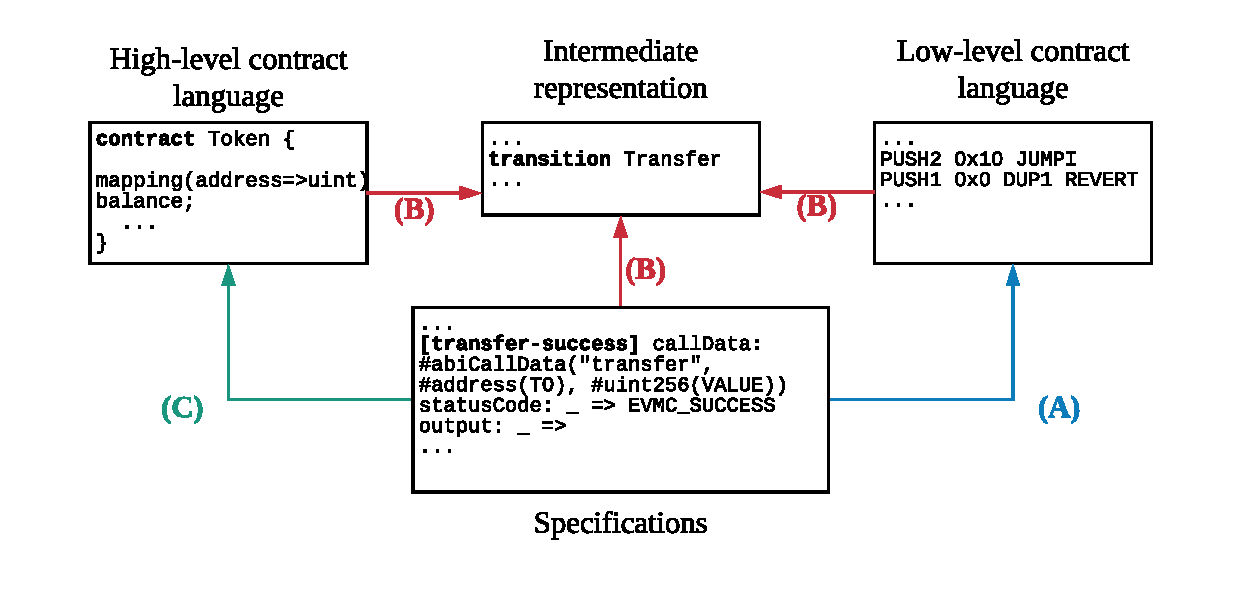
\includegraphics[width=\textwidth]{fig/Verification.pdf}
\caption{Different approaches of verification tools regarding their source for deriving a model or a set of formulas representing the system. Methods listed in \textbf{(A)} directly verify properties from the model or set of formulas from the low-level code. \textbf{(B)} describes tools using an IR from a high-level langauge or from the low-level code to verify the system. Last, \textbf{(C)} describes methods for verifying properties directly from the high-level code.}
\end{figure}

\subsection{Summary}

Verification efforts can be characterised by five criteria \cite[173]{Huth2004}. From these, we adopt three and fixate the other two. 
The application domain concerns smart contracts on a deterministic distributed ledger.
On these ledgers smart contracts are \emph{immutable}, hence, verification before or during, but latest, before deployment, is desirable. Otherwise, they can only be used to find bugs that are already introduced in the software and mostly requires significant efforts to resolve or update the contracts.
Additionally, we included the language that is covered by the specific tool as well as the availability of source code.
This leaves us with the following criteria.
Table \ref{tab:model} presents an overview of the tools we have considered for this survey.

\begin{itemize}
\item \emph{Approach}: In proof-based verification, the system is represented by a set of formulas, while in model-based verification the system is a model. Properties are represented as formulas. The goal is to either proof (proof-based) or to compute whether a model (model-based) satisfies these properties. Proof-based methods typically derive a formal definition of the distributed VM and then try to verify properties of a smart contract. Model-based methods build a model directly from the smart contract and verify the properties with an implicit model of the VM.
\item \emph{Automation}: Fully automated approaches have a set of properties and automatically build a model for the system based on an input (like the source code). Partial automation typically requires defining properties or using a proof-assistant (e.g. Coq or Isabelle/HOL) to define and check proofs.
\item \emph{Coverage}: Property-based verification is concerned with selected parts of the system, while full covers the system as a whole.
\item \emph{Languages}: Lists the languages that are currently, as of September 2018, supported by the methods. Some of the general tools like Lem, F*, K, and Coq can be used for any languages. However, we only list the ones where current research is done.
\item \emph{Source}: Indicates whether the tools and the verification work is available as open source. This criterion is interesting to verify results, experiment with the available tools, and potentially expand them.
\end{itemize}

\begin{table*}
\renewcommand{\arraystretch}{1.3}
\centering
\caption{Overview of model and proof-based verification tools for smart contracts.}
\label{tab:model}
\begin{tabularx}{\textwidth}{XXXXXXr}
\toprule
\textbf{Tool} & \textbf{Approach} & \textbf{Automation} & \textbf{Coverage} & \textbf{Languages} & \textbf{Source} & \textbf{Ref.} \\ \toprule
\emph{Securify} & model & full & full & Solidity, EVM & open & \cite{Tsankov2017} \\
\emph{Mythril} & model & full & property & EVM & open & \cite{Mueller2018} \\
\emph{Oyente} & model & full & property & Solidity, EVM & open & \cite{Luu2016,Albert2018} \\
\emph{ZEUS} & model & full & property & Solidity, Go, Java & closed\textsuperscript{\dag} & \cite{Kalra2018} \\
\emph{ECF} & model & full & property & EVM & open & \cite{Grossman2017} \\
\emph{Maian} & model & full & property & EVM & open & \cite{Nikolic2018} \\ \midrule
\emph{$\mathbb{K}$} & proof & partial & full & EVM, IELE & open & \cite{Hildenbrandt2017,Park2018} \\
\emph{Lem} & proof & partial & full & EVM & open & \cite{Hirai2017,Amani2018} \\
\emph{Coq} & proof & partial & partial\textsuperscript{\ddag} & Scilla, Michelson & open & \cite{Sergey2018,DynamicLedgerSolutions2017} \\
\emph{F*} & proof & partial & partial\textsuperscript{\ddag} & EVM & open & \cite{Bhargavan2016,Grishchenko2018} \\
\bottomrule
\end{tabularx}
\justify
\textsuperscript{\dag} We were not able to find open source code. \\
\textsuperscript{\ddag} Theoretically these tools have a full coverage. However, implementation is as of September 2018 not completed.
\end{table*}




\subsection{Model-based methods}
Model-based methods mostly arise from the need to check contracts for known vulnerabilities. After the DAO and Parity vulnerabilities were known, tools were developed to find similar patterns in other contracts.

\paragraph{Tools:}
Securify is a domain-specific model checker for smart contracts \cite{Tsankov2017}. It compiles EVM bytecode to semantics facts and then uses a DSL to define compliance and violation patterns to verify the semantic facts. The properties are build using Datalog, a logic language. It classifies behaviours of a contract in compliance (matched by compliance properties), violations (matched by violation properties) and warnings (matched by neither). Securify is only available as a web-service to verify smart contracts.

Mythril is a symbolic execution of EVM bytecode \cite{Mueller2018}. EVM bytecode is disassembled into a Mythril object, and propositional logic is used to reason about the state space represented as a graph. It is based on the IR LASER \cite{Mueller2018LASER}.

Oyente \cite{Luu2016} and its proposed extension EthIR \cite{Albert2018} build a model from EVM bytecode to verify pre-defined properties. It is one of the first tools to allow verification of selected properties based on a simulation of the EVM. Properties include transaction ordering dependencies, timestamp dependencies, mishandled exceptions, and reentrancy.

ZEUS is an exception to the other tools as it uses Solidity or Java and Go (as Hyperledger Fabric contracts) as its basis for evaluation \cite{Kalra2018}. It compiles these contracts into an abstract language. Next, properties defined in XACML are used to reason about the contract. The properties together with the abstract language contract get translated to LLVM bitcode for symbolic execution and verification of the properties.

Effectively Callback Free (ECF) objects are a unique property that is analysed for Ethereum smart contracts\cite{Grossman2017}. A callback method opens up the possibility to change the state of an object (contract) from an external object (contract), which makes reasoning difficult. The authors show that most Ethereum contracts are ECF except for those subject to the vulnerabilities similar to the DAO bug (also referred to reentrancy in other work).

Maian works by symbolic execution of a model of EVM bytecode contracts to find trace vulnerabilities \cite{Nikolic2018}. These vulnerabilities include contracts that leak Ether to unintended parties, can be killed by arbitrary users or lock Ether that cannot be received. They apply their method to verify these properties in real-world contracts.

\paragraph{Automation:} Model-based tools are automated. They usually use an SMT solver (e.g. Z3) to explore the fulfilment of violation of properties. Automation offers a significant advantage as the pre-defined properties in the tool can easily be verified on other contracts. Moreover, Securify, Oyente, and Mythril are available as a web-service. This allows developers to check their contracts without the need to install dependencies for model checking locally.

\paragraph{Coverage:} Most model-based tools verify selected properties. In \cite{Atzei2017} and \cite{Luu2016}, the authors offer a classification of possible vulnerabilities. These vulnerabilities build the basis for the properties to check as the tools try to identify violations or conformance of those patterns to flag a contract as vulnerable. Further work tries to build a semantic definition of security based on those vulnerabilities \cite{Grishchenko2018}. The presented tools flag contracts as vulnerable that match properties. Securify additionally gives a warning if none of its conformance or violation patterns matches. However, other tools do not indicate such warnings. Hence, contracts might still be vulnerable even if no properties were triggered (i.e.\ false negative).

\paragraph{Languages:} Ethereum is the most popular platform for finding such vulnerabilities. Notably, other languages like Bitcoin Script seem to be quite restrictive leading to less of a need to automatically verify security properties. The majority of the tools use the EVM bytecode to derive a model of the contract. ZEUS is an exception as it builds the model based on higher-level languages such as Solidity or Java and Go. Moreover, most models do not implement all EVM opcodes. Hence, vulnerabilities might remain undetected as not all contracts can be fully verified.

\paragraph{Source:} Most tools are open source and their code is available online. All tools have a description in a paper or technical report that gives details about their internals. They offer extensions by creating new properties for verification. Except for Securify and ZEUS, tools can be cloned locally, and additional properties can be added.


\subsection{Proof-based methods}
The proof-based methods arise from the need to proof contracts secure. This requires a formal semantics of the VM and the low-level language. Overall, these methods are used to prevent future vulnerabilities but depend on an exact definition of properties and rigorous formal semantics.

\paragraph{Tools:} K is a general purpose framework for defining programming languages \cite{Rosu2007}. It is used to build a K representation of the EVM, called KEVM \cite{Hildenbrandt2017}. This VM has been successfully tested against the official test-set of the Ethereum Foundation for any new EVM implementation. Contracts like ERC20 can be specified in K as well \cite{Park2018}. The contract can be formally verified using the compiled bytecode, the K contract, and the KEVM virtual machine. Moreover, K is used to defined IELE \cite{Kasampalis2018} and can be used to verify contracts based on this VM.

Lem is used to defining language semantics and can be used to derive implementations in OCaml and enable proof-based verification using Coq, HOL4, or Isabelle/HOL \cite{Mulligan2014}. The EVM has been defined in Lem and subsequently contracts verified using the semantic definition \cite{Hirai2017}. This work is extended by \cite{Amani2018}. The Lem definitions and smart contract verification are pursued by \citeauthor{Hirai2018} at the Ethereum Foundation \cite{Hirai2018}.

Coq is an interactive theorem prover that can be used for any language theoretically. In practice, Scilla is defined in Coq, and there are ongoing efforts to verify Scilla contracts \cite{Sergey2018}. Further, Coq is intended to be used together with the Michelson language \cite{DynamicLedgerSolutions2017}.

\citeauthor{Bhargavan2016} propose to convert Solidity and EVM bytecode to F* \cite{Bhargavan2016}. This can then be used to verify properties in the contract and obtain a secure implementation. However, the work does not present a full implementation.
Further, a complete small-step semantics of the EVM semantics is presented in \cite{Grishchenko2018}. Based on this semantics the authors have implemented in large parts the EVM in F*. F* has then been compiled to OCaml code to verify the EVM implementation against the official Ethereum test suite.

\paragraph{Automation:} Proof-based tools are partially automated. The Lem, K, F* semantics are concentrating on creating the distributed VM that executes the smart contracts. Automation can be reached by defining properties contracts should fulfil. This is partly done by the ERC20 efforts in K and the Deed contract in Isabelle/HOL. However, it is desirable to define the functionality of a contract and then verify its correctness rather than finding selected vulnerabilities. The verification of the properties is then done using an SMT solver (in K) or using an interactive theorem prover (Lem, Coq, F*).

\paragraph{Coverage:} The desired coverage of those tools is the full contract. By giving a formal specification of the contract functionalities, a contract can be deemed correct. This approach is beneficial for common standards (e.g. ERC20 or ERC721). Selected properties might still be defined instead of the full contract. This approach can also have short-comings as a formally verified contract might contain bugs due to incomplete or inaccuracies in the VM semantics \cite{Hirai2016}.

\paragraph{Languages:} Major work efforts are taken in building a formal semantics of the EVM (K, Lem, F*). K and Lem are complete and derived implementations have been tested against the EVM test suite corpus. The F* implementation is partially complete. While the EVM semantic is defined after its implementation, other languages take a different approach. IELE, Scilla, and Michelson are designed with formal verification in mind. Hence, their semantics are currently developed and in the future formal verification should be comparably easy. Further, their formal semantics approach helps to build verified compilers.

\paragraph{Source:} All tools are open-source. The K framework has quite extensive documentation and examples available, followed by the work on Lem and Isabelle/HOL. The Coq and F* methods are somewhat new, and documentation is sparse. Also, the semantics are incomplete making those tools not yet practical to use for smart contract verification.


\section{Discussion}
\label{discuss}

High-level languages for smart contracts are designed and improved to promote safe smart contracts.
This is achieved by making state changes explicit by using an FSM/automata approach. 
They typically restrict the instruction set by only allowing finite loops and recursion.
Moreover, the code should be as explicit as possible by preventing function overloading, creating explicit types for assets and units, and promoting pure functions.
Intermediary languages are developed with formal verification and optimisations in mind.
This is an attempt to bring best practices from software engineering and language theory to distributed ledgers.
Low-level languages are built to allow formal verification and at the same time give a run-time optimised execution on a distributed ledger.

Verification efforts include categorising and defining security properties for smart contracts, developing model-based tools to verify that contracts are not vulnerable to known bugs, and formal semantics with the intention to prove compliance of a contract implementation to an abstract specification.

\subsection{Related work}
Security of smart contracts is a widely discussed subject.
\citeauthor{Seijas2017} survey smart contracts for distributed ledger with a focus on Bitcoin, Ethereum, and Nxt \cite{Seijas2017}.
They provide an overview of the interactions between smart contracts and the underlying ledger.
Further, they sketch selected approaches to create smart contracts and allow for more security.
In an empirical analysis, the use cases of smart contracts in Bitcoin and Ethereum are discussed\cite{Bartoletti2017}.
The authors introduce a taxonomy of smart contracts according to usage categories and design patterns in Ethereum smart contracts.

The call graph by Ethereum contracts is evaluated in \cite{Frowis2017}.
An analysis of security vulnerabilities of smart contracts with a focus on the EVM is presented in \cite{Luu2016} and \cite{Atzei2017}.
\citeauthor{Grishchenko2018} extend this work by introducing a formal semantic definition of safety properties of smart contracts.

\citeauthor{Sergey2018} present a brief overview and comparison of 13 smart contracts languages in section five \cite{Sergey2018}. \citeauthor{Tsankov2017} include an overview and comparison to related work on smart contract verification including an evaluation of Securify, Oyente, and Maian \cite{Tsankov2017}.

Apart from language design and verification, other methods are proposed to increase the security of smart contracts. Hydra is a bug-bounty and security protocol for smart contracts \cite{Breidenbach2018}. The idea is to replicate a smart contract logic in different implementations that need to reach consensus over state-changing executions. This sacrifices liveness for security and can be used for critical applications.

NECTAR is an extension to Bitcoin's UTXO model and script set \cite{Covaci2018}. Smart contracts in this setting include a proof that can be checked along its execution. Other nodes in the network need to check the proof instead of re-executing the code to verify that the smart contract has been executed correctly.

Further, game theory and Markov decision process (MDP) can be used to model users interacting with a smart contract \cite{Bigi2015}. By applying both methods, the authors validate a protocol build on a smart contract. In that case, external factors like the users are considered explicitly as players in a game.

%\subsection{Future work}
%Formal semantics

%Verified compilers

%Automated verification

\section{Conclusion}
\label{conclusion}
An overview of smart contracts and verification methods is presented.
Languages are developed and improved to allow easier verification by defining formal semantics. Also, secure patterns like explicit state transitions and restricted instructions are applied. Verification efforts concentrate on finding known vulnerabilities and formally defining smart contract logic to verify implementations.

We note three areas of future work. Formal semantics are being adopted for low-level languages, and selected IRs have been designed from a formal semantics. However, high-level languages with full formal semantics are just being developed.
Formal semantics on all levels of languages is a requirement to develop verified compilers \cite{Hirai2017}. Verified compilers and formal semantics can then be used to build automated proof-based verification methods.

% Smart contracts are a new type of programs that have direct access to currency and are executed on a global distributed network. 

\printbibliography

\end{document}
